\section{Introduction}

% REVISION: addresses W1
Self-supervised world models that learn dynamics in latent space are an increasingly practical route to goal-conditioned control from pixels. Recent JEPA-style models train without reward supervision and can achieve high planning success on selected manipulation benchmarks.

Figure~\ref{fig:overview} summarizes the audit pipeline: endpoint ranking tests fixed artifacts, pool ranking tests the candidates produced by the optimizer, and selection metrics test the action that would actually execute.

\begin{figure*}[t]
\centering
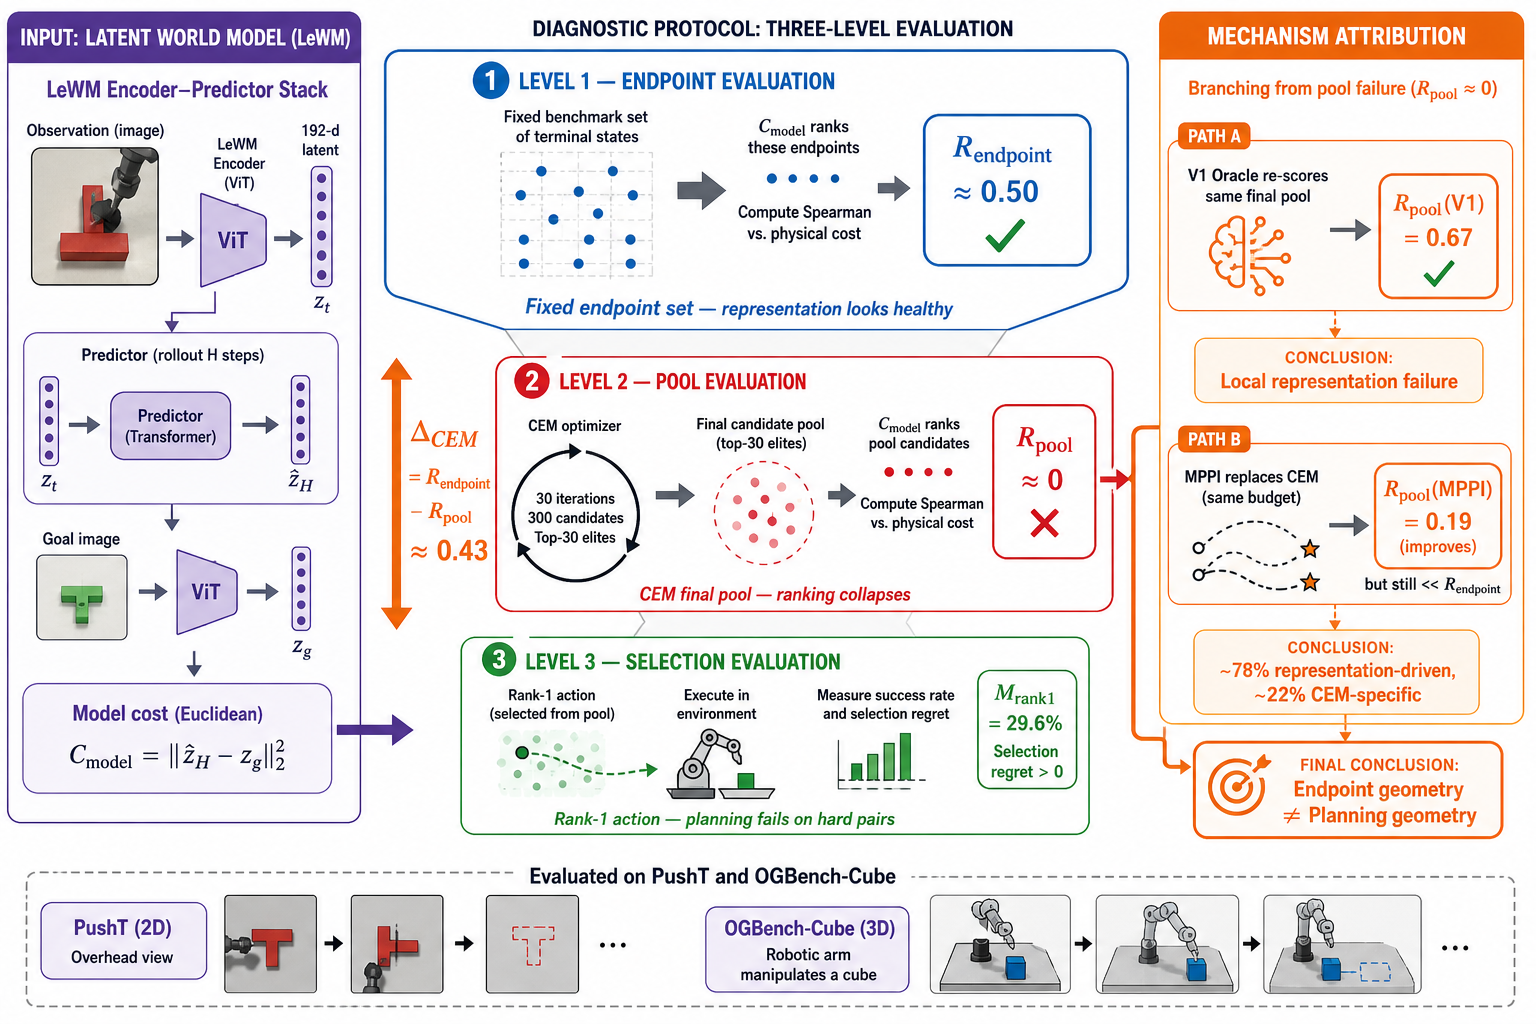
\includegraphics[width=\textwidth]{figures/fig_overview.png}
\caption{Overview of the three-level diagnostic protocol for auditing latent world models. \textbf{Left:} The LeWM encoder-predictor stack maps observations to 192-dimensional latents and scores candidates by Euclidean terminal cost $C_{\text{model}} = \|\hat{z}_H - z_g\|_2^2$. \textbf{Center:} Three evaluation levels expose endpoint-planning decoupling. Level~1 (endpoint evaluation) measures $R_{\text{endpoint}} \approx 0.50$ on a fixed benchmark---the representation appears healthy. Level~2 (pool evaluation) measures $R_{\text{pool}} \approx 0$ inside the CEM final pool---ranking collapses, yielding $\Delta_{\text{CEM}} \approx 0.43$. Level~3 (selection evaluation) records rank-1 success ($M_{\text{rank1}} = 29.6\%$) and selection regret. \textbf{Right:} Mechanism attribution branches from the pool-level failure. Actual-terminal V3 scoring raises $R_{\text{pool}}$ to 0.26, while V1 physical scoring reaches 0.67, showing that predictor rollout contributes but learned terminal-latent geometry remains limiting. Path~B replaces CEM with MPPI soft weighting, improving $R_{\text{pool}}$ to 0.19 but still far below $R_{\text{endpoint}}$. \textbf{Bottom:} The protocol is evaluated on PushT (2D pushing) and OGBench-Cube (3D manipulation).}
\label{fig:overview}
\end{figure*}

LeWM is one such model \citep{lewm2025}. Panels~\ref{fig:decoupling_evidence}a--c illustrate the core finding: endpoint ranking can appear structured while CEM-pool ranking collapses. Figure~\ref{fig:motivation}a shows the long-horizon failure on PushT: success falls from 96\% at a 25-step goal offset to 10\% at 100 steps. LeWM trains with next-embedding prediction and SIGReg regularization; its 18.0M-parameter encoder-predictor stack produces 192-dimensional latent states and rolls candidate action sequences forward. At inference, CEM scores the predicted terminal latent $\zhatH$ against a goal latent $\zgoal$ by Euclidean latent distance $\Cmodel$. LeWM also reports up to $48\times$ faster planning than DINO-WM \citep{dinowm2024}. The question is where the long-horizon failure originates.

\begin{figure*}[t]
\centering
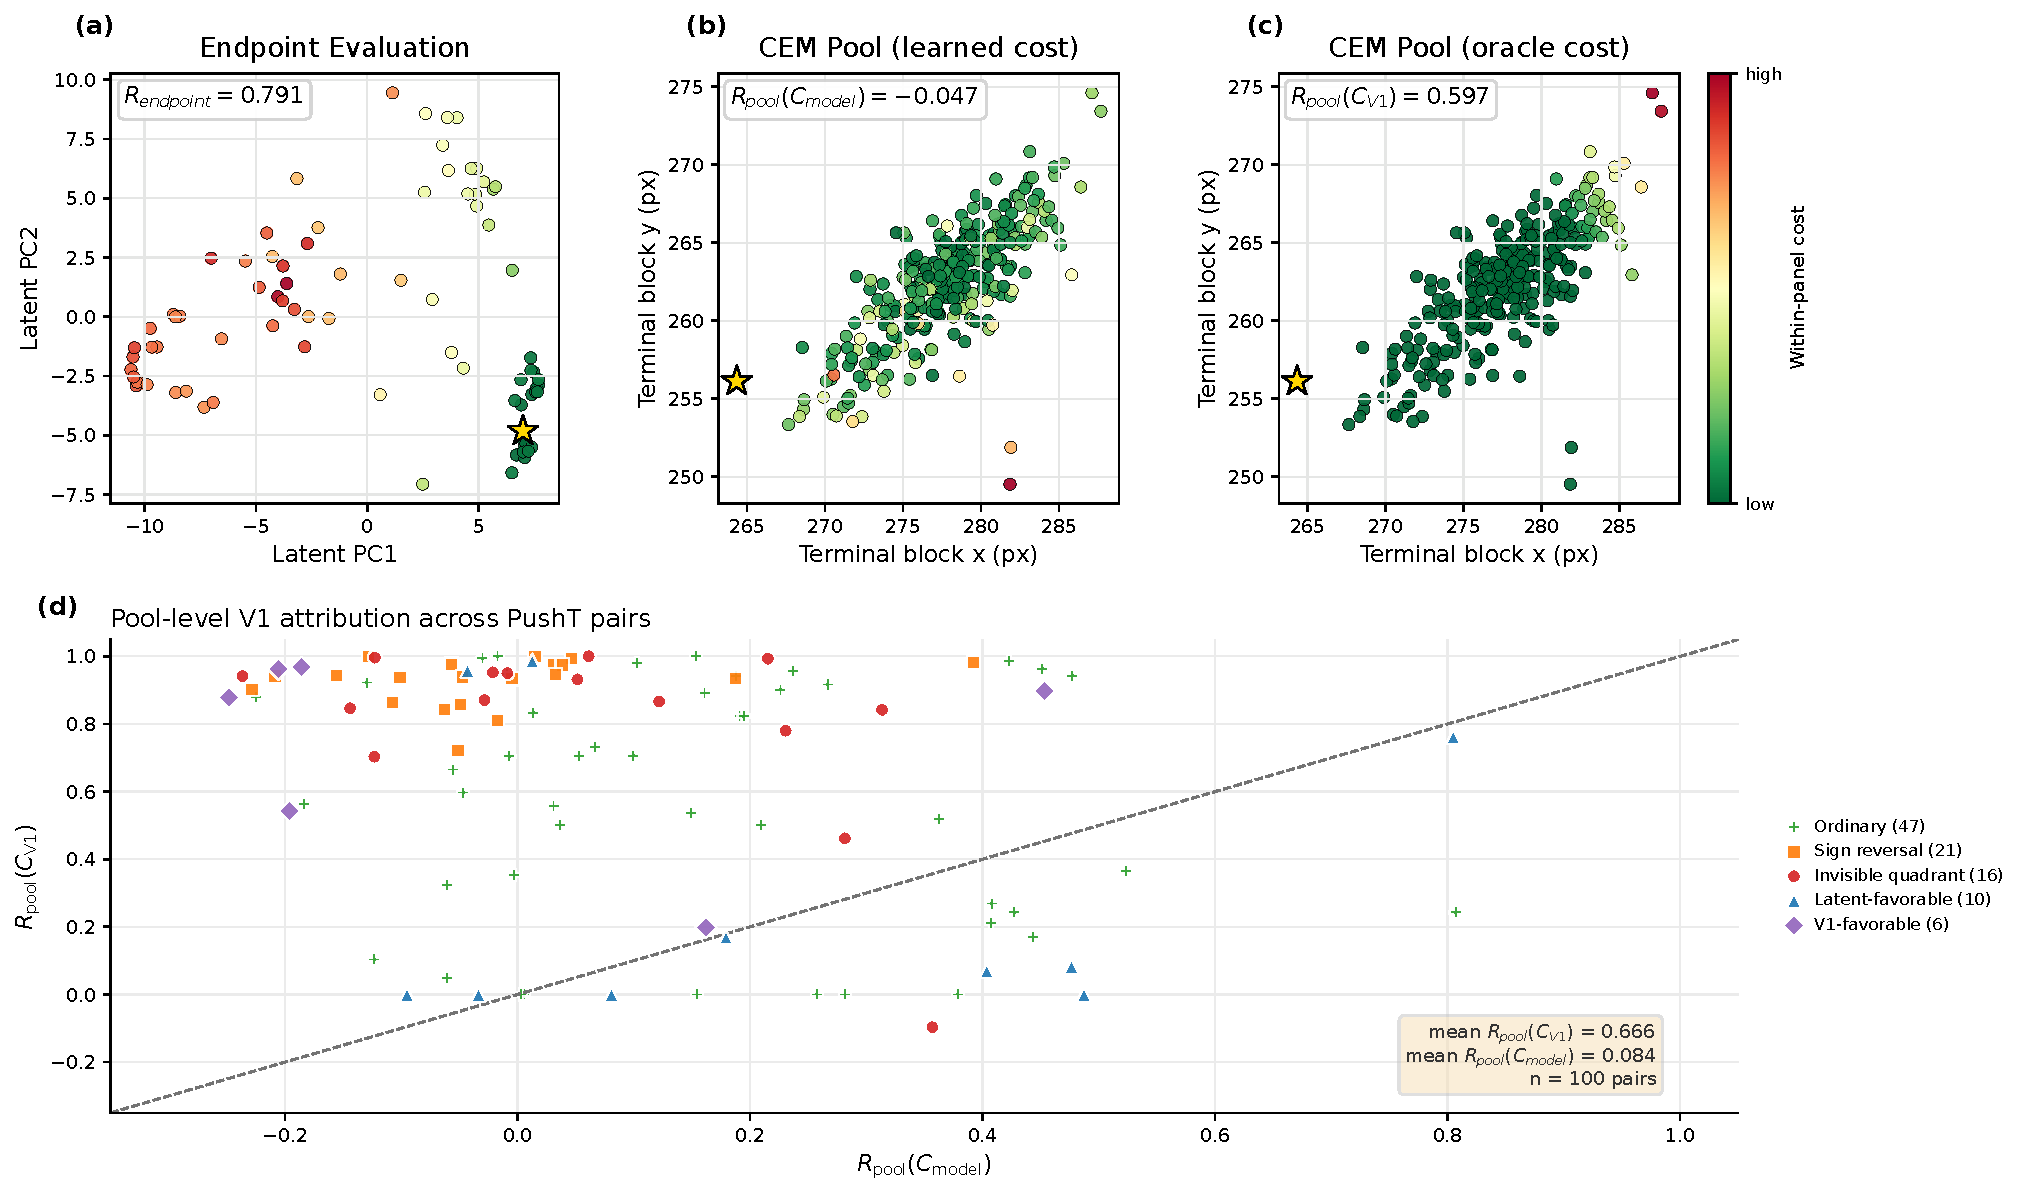
\includegraphics[width=\textwidth]{figures/fig2_combined.pdf}
\caption{Endpoint-planning decoupling on PushT. \textbf{(a)}~On a fixed endpoint set, the learned latent cost produces a spatial gradient ($\Rendpoint=0.79$). \textbf{(b)}~In the CEM final pool, the same cost scrambles the ranking in physical space ($\Rpool(\Cmodel)=-0.05$). \textbf{(c)}~The V1 oracle cost recovers the gradient on the same pool ($\Rpool(C_\mathrm{V1})=0.60$). \textbf{(d)}~Pool-level attribution across all 100 pairs: V1 outperforms the learned cost in every subset, and Section~4.4 adds actual-terminal V3 scoring to separate predictor rollout error from terminal-latent geometry.}
\label{fig:decoupling_evidence}
\end{figure*}

The standard diagnostic toolkit first examines the representation: does the latent state preserve task-relevant information, and does latent distance track physical task cost? Endpoint metrics answer these questions by freezing the action-generation problem. They compare terminal states after the fact, then ask whether latent distances rank them like physical costs. This isolates representation quality from the stochastic planner and yields a stable metric for comparing models, seeds, and projection dimensions. On these tests, LeWM does not fail visibly: learned latent distances correlate with physical costs on fixed endpoint sets, random projections preserve much of the 192-dimensional ranking signal, and predictor rollouts retain much of this geometry in aggregate. The resulting puzzle is narrower than encoder collapse: endpoint-only metrics do not explain why CEM fails at long horizons.

The missing object is the candidate pool produced by CEM itself. CEM does not choose from a fixed endpoint benchmark. It samples actions, predicts terminal latents, selects elites, and updates its proposal distribution. After 30 iterations, the ranking that matters is local: the ranking inside the final 300-candidate pool, not the global endpoint ranking. We denote the endpoint rank correlation as $\Rendpoint$ and the final-pool rank correlation as $\Rpool$, and measure their difference as $\DeltaCEM=\Rendpoint-\Rpool$. In PushT, this gap reaches 0.43 at projection dimension $m=64$. A similar gap of 0.57 appears in OGBench-Cube. The rest of the paper shows that this endpoint-pool split persists across matched protocols and explains why endpoint ranking alone cannot predict CEM behavior.

This finding emerged from a pre-registered audit, not a single post-hoc analysis. The audit began with an encoder-collapse hypothesis, but the representation retained endpoint-ranking signal. Cost-landscape mismatch was closer yet still incomplete, so the final framing separated endpoint geometry from planning geometry. Each reset followed a locked decision tree, fixed pair sets, and pre-specified continuation rules. The same discipline kept the negative results useful: each failed repair removed a simpler explanation and narrowed the account.

% REVISION: addresses W1
Our empirical claims apply to LeWM with Euclidean terminal latent costs under CEM-style optimization, evaluated on PushT and OGBench-Cube. The evaluation principle is broader, but it should be applied with the same instrumentation: endpoint metrics are not wrong; they measure whether a representation carries task information, not whether an iterative planner can use that information during search. Planning evaluation should therefore include the distributions produced by the optimizer itself. We propose a minimal reporting protocol with three views. Report endpoint metrics on a fixed benchmark set. Report pool metrics on the candidates produced by the planner. Report selection metrics for the action that is actually executed. For latent planners with terminal-cost objectives, this audit is directly applicable when final candidate pools can be saved and an evaluation-time physical cost is available. The goal is a planning-compatible test of geometry, not another endpoint-only score.

\begin{figure}[t]
\centering
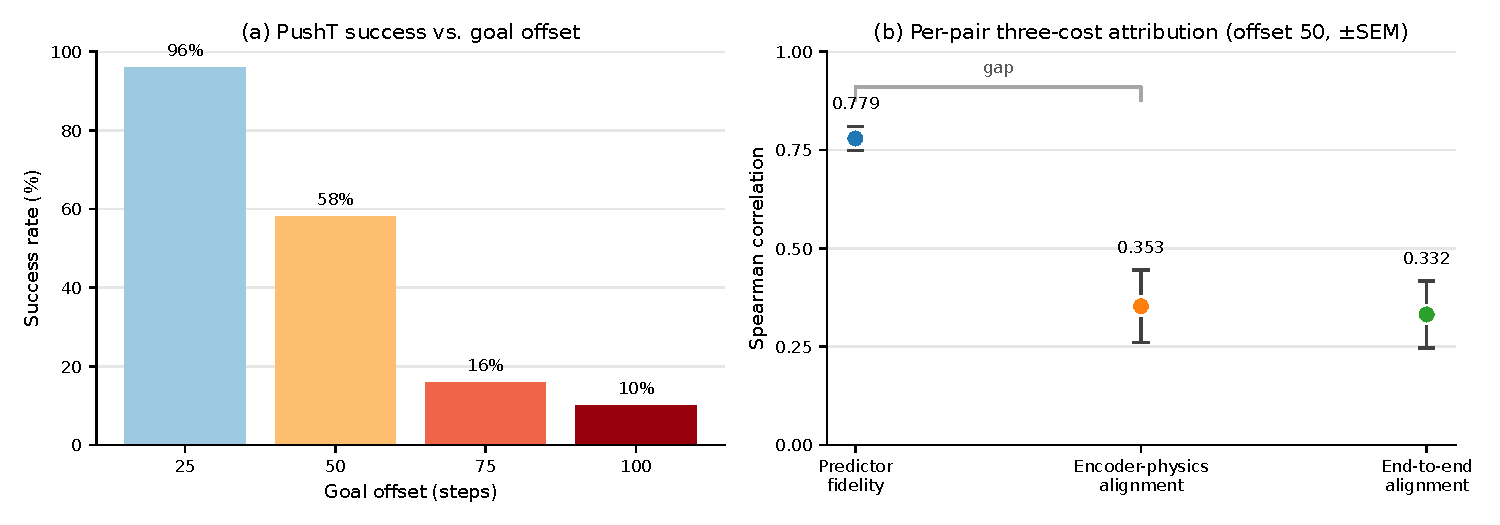
\includegraphics[width=\textwidth]{figures/fig2_enhanced.pdf}
\caption{Motivating evidence for the endpoint-planning gap. \textbf{(a)}~PushT planning success drops sharply with goal offset, from 96\% at offset~25 to 10\% at offset~100. \textbf{(b)}~Per-pair three-cost attribution at offset~50 shown as a dot plot ($\pm$\,SEM, $n=30$ pairs). Predictor fidelity is high (mean Spearman 0.779), but encoder-physics alignment is weak and heterogeneous (0.353), so end-to-end alignment is also low (0.332). The gap between predictor fidelity and encoder-physics alignment motivates the distinction between endpoint geometry and planning geometry developed in Section~4.}
\label{fig:motivation}
\end{figure}

The rest of the paper is organized as follows. Section~2 introduces LeWM and CEM planning. Section~3 presents the audit framework. Sections~4--6 report the main findings. Sections~7--8 discuss implications and limitations. Figure~\ref{fig:decoupling_evidence} previews the central finding.
